\documentclass{article}
\usepackage[utf8]{inputenc}
\usepackage{graphicx}
\usepackage{multirow}

\title{Antworten zu Aufgabenblatt 1}
\date{2019-06-04}
\author{Rebecca, Joshua, Alexander}

\begin{document}
    \maketitle
    \newpage
    \section{Aufgabenblatt 1}
    \subsection{Aufgabe 1}
        \subsubsection{a)}
        Die Reihenfolge in welcher die IDs der Threads ausgegeben werden ist jedes Mal unterschiedlich und ist auch nicht vorherzusagen.
        
        \subsubsection{b)}
        Gemessen wurde auf dem i82sn02. Für die manuelle Parallelisierung wurde atomic verwendet. Diese Messung wurde nach 4 Threads aufgehört da sich die Rechenzeit stark erhöht hat. Für das Parallelisieren mit Reduktion ist das maximales Speedup $ \sim 8 $.\\
        Bei 16 und 32 Threads verschlechtert sich die Beschleunigung im Gegensatz zu 8 Threads bei kleineren N. Das könnte am Overhead der Verarbeitung der Threads liegen.
        
	\begin{tabular}{|l|l|r|r|r|}
		\hline
		- & Number of Threads & N & Time (s) & Speedup \\
		\hline
		sequential & 1 & 1000 & 0.002 & - \\
		& 1 & $10^{7}$ & 0.239 & - \\
		& 1 & $10^{8}$ & 2.388 & - \\
		& 1 & $10^{9}$ & 23.642 & - \\
		& 1 & $10^{10}$ & 239.508 & - \\
		\hline
		manual & 2 & 1000 & 0.002 & 1 \\
		 & 2 & $10^{7}$ & 0.634 & - \\
		 & 2 & $10^{8}$ & 6.461 & - \\
		 & 2 & $10^{9}$ & 52.989 & - \\
		 & 4 & $10$ & 0.003 & - \\
		 & 4 & $10^{7}$ & 1.214 & - \\
		 & 4 & $10^{8}$ & 13.491 & - \\
		 & 4 & $10^{9}$ & $\sim$ 120 & - \\
		\hline
		reduction & 2 & 1000 & 0.002 & 1 \\
		 & 2 & $10^{7}$ & 0.121 & 1.9 \\
		 & 2 & $10^{8}$ & 1.188 & 2 \\
		 & 2 & $10^{9}$ & 11.845 & 1.9 \\
		 & 2 & $10^{10}$ & 118.204 & 2 \\
		 & 4 & 1000 & 0.003 & - \\
		 & 4 & $10^{7}$ & 0.062 & 3.9 \\
		 & 4 & $10^{8}$ & 0.595 & 4 \\
		 & 4 & $10^{9}$ & 5.959 & 3.9 \\
		 & 4 & $10^{10}$ & 59.183 & 4 \\
		 & 8 & 1000 & 0.003 & - \\
		 & 8 & $ 10^{7} $ & 0.032 & 7.5 \\
		 & 8 & $ 10^{8} $ & 0.299 & 7.9 \\
		 & 8 & $ 10^{9} $ & 2.967 & 7.9 \\
		 & 8 & $10^{10}$ & 29.689 & 8.0 \\
		 & 16 & 1000 & 0.003 & - \\
		 & 16 & $ 10^{7} $ & 0.040 & 5.9 \\
		 & 16 & $ 10^{8} $ & 0.318 & 7.5 \\
		 & 16 & $ 10^{9} $ & 3.028 & 7,8 \\
		 & 16 & $10^{10}$ & 29.674 & 8.1\\
		 & 32 & 1000 & 0.004 & - \\
		 & 32 & $ 10^{7} $ & 0.037 & 6.4 \\
		 & 32 & $ 10^{8} $ & 0.305 & 7,8 \\
		 & 32 & $ 10^{9} $ & 2.987 & 7.9 \\
		 & 32 & $10^{10}$ & 29.551 & 8.1 \\
		\hline
	\end{tabular}

	\newpage
        \subsubsection{c)}
        
        Die Messbedingungen waren gleich wie im Aufgabenteil b). Die Werte für das Speedup unterscheiden sich nicht groß von den oben gemessenen.\\
        
        \begin{tabular}{|l|r|r|r|}
        	\hline
        	 Auflösung N & No. Threads &  Time (s) & Speedup \\
        	 	\hline
        	 1000& 1 &  4.411 & - \\
        	 1000& 2 &  2.228 & 1.980 \\
        	 1000& 4 &  1.122 & 3.931 \\
        	 1000& 8 &  0.563 & 7.835\\
        	 1000& 16 &  0.567 & 7.780 \\
        	\hline
        	2000& 1 & 17.625 & - \\
        	2000& 2 &  8.896& 1.981 \\
        	2000& 4 &  4.493& 3.923 \\
        	2000& 8 &  2.254& 7.819 \\
        	2000& 16 &  2.248& 7.840 \\
        	\hline
        	4000& 1 & 71.761 & - \\
        	4000& 2 &  35.559 & 2.010 \\
        	4000& 4 &  17.952& 3.997 \\
        	4000& 8 &  8.978 & 7.991\\
        	4000& 16 &  8.980 & 7.991 \\
        	\hline
        	5000& 1 &  110.143 & - \\
        	5000& 2 &  55.564 & 1.982 \\
        	5000& 4 &  27.951 & 3.94 \\
        	5000& 8 &  13.995 & 7.870 \\
        	5000& 16 &  14.020 & 7.856\\
        	\hline
        \end{tabular}
	\begin{center}
		
\includegraphics[width=0.6\linewidth]{Aufgaben-Ressourcen/normal-1000.jpg}	
	\end{center}

	\begin{center}
		
\includegraphics[width=0.4\linewidth]{Aufgaben-Ressourcen/critical-1000.jpg}\quad
\includegraphics[width=0.4\linewidth]{Aufgaben-Ressourcen/critical-1000-1000.jpg}
		\\[\baselineskip]
		\includegraphics[width=0.4\linewidth]{Aufgaben-Ressourcen/critical-10000-1000.jpg}\quad\includegraphics[width=0.4\linewidth]{Aufgaben-Ressourcen/critical-10000-1000.jpg}
	\end{center}


    \subsection{Aufgabe 2}
    	\subsubsection{a)}
		\begin{enumerate}
			\item Example: \\
				Es besteht eine Race-Condition auf dem Array a über Index i,
				bei ungünstiger Ausführungsreihenfolge der Threads kann es dazu kommen,
				das a[i] durch einen Thread geschrieben wird und von einem anderen Thread versucht wird, darauf in der nachfolgenden Anweisung lesend zuzugreifen.
				Um dieses Problem zu lösen können zwei for-Schleifen verwendet werden.
				Eine schreibt alle Werte in Array a und die zweite schreibt alle Werte unter Zugriff auf Array a in Array b. 
				Beide Schleifen werden jeweils getrennt parallelisiert.
			\item Example: \\
				Threads exisiteren hier in der gesamten parallelen Region.
				Das nowait-Statement der ersten parallelisierten For-Schleife bewirkt, dass Threads bereits die nächste parallelisierte Schleife bearbeiten können, wenn sie ihren Teil der ersten Schleife fertig verarbeitet haben.
				Dies führt zu einer Race-Condition auf das Array a mit Index i, ähnlich zu Example 1.
				Mit dem entfernen des nowait-Statements der ersten for-Schleife warten alle Threads wieder auf die implizite Barriere bis alle Threads fertig sind und es kann Problemlos auf die geschriebenen Werte in Array a zugegriffen werden.
			\item Example: \\
				Hier ist die Variable x zunächst global definiert und wird somit implizit zwischen den Threads geshared. 
				Somit besteht eine Race-Condition auf x da die Threads unabhängig voneinander sowohl lesend als auch schreibend auf x zugreifen.
				Indem man x explizit als private deklariert, erhält jeder Thread seine eigene Kopie der Variable und es besteht keine Race-Condition mehr.
			\item Example: \\
				f ist global definiert und wird durch jeden Thread private gesetzt. 
				Allerdings erhält jeder Thread eine uninitialiserte Kopie der Variable f, was bedeutet das dass initialisieren mit dem Wert 2 vor der Schleife nur für den Master-Thread sichtbar ist.
				Um diese Initialiserung auch für alle übrigen Threads sichtbar zu machen, ist es erforderlich, f mittels firstprivate zu deklarieren.
				Des weiteren wird der Wert von x nicht aus der parallelen Region wieder rausgeschrieben, sondern gelöscht. 
				Wodurch der zuletzt geschriebene Wert innerhalb der parallelen Region in x nach außen hin nicht sichtbar ist.
				Um deses Verhalten zu erreichen, muss x als lastprivate deklariert werden.
			\item Example: \\
				Hier besteht eine Race-Condition auf die Variable sum. 
				Da mehrere Threads versuchen hier den alten Wert von Sum zu lesen, den i-ten Wert aus b ausfzuaddieren und damit sum wieder zu überschreiben, ist nicht garantiert, dass sum am Ende den korrekten Wert enthält.
				Indem man das auslesen, aufaddieren und zuweisen mittels critical-Konstrukt schützt, ist garantiert das immer nur ein Thread den Wert überschreiben kann.
				Allerdings ist die gesamte Schleife dann gleichbedeutend mit einer Sequenziellen Ausführung.
		\end{enumerate}

		\subsubsection{b)}
			Werden Matrizen in C zeilenweise im Speicher hinterlegt, ist es zur optimalen Ausnutzung von Caching-Effekten ideal, wenn auch zeilenweise über Einträge der Matrix iteriert wird.
			Dadurch läd der Prozessor bei einem Cache-miss auf einen Eintrag nicht nur den einzelnen Eintrag in den Cache, sondern direkt mehrere nachfolgende Einträge, was weniger Zugriffe auf den RAM zu folge hat und somit insgesamt die Performance verbessert.
			Wird jedoch spaltenweise über eine Matrix iteriert, müssen für einen Zugriff auf das (i+1)-te Element alle n-Einträge nach i ausgelassen werden. 
			Bei entsprechend großen Matrizen werden die mit in den Cache geladenen Elemente garnicht benötigt.
			Jeder Zugriff entspricht somit einem Cache-miss, was wiederum einen Speicherzugriff zur folge hat und somit die gesamte Performance negative beeinflusst.
			
			Der klassische IJK-Algorithmus zur Matrixmultiplikation iteriert in der inneren K-Schleife für die rechte Matrix B für jede Addition+Multiplikation über die Spalten.
			Zum besseren Ausnutzen der Cache-Effekte kann durch vertauschen der zwei Schleifen J und K, auch bekannt als IKJ-Optimierung, eine Verbesserung der Performance erzielt werden.
			So wird in der inneren J-Schleife nur über die Spalten aus B und C iterriert und die K-Schleife iteriert über die Spalten in A.

			Da der einzelne Eintrag in A der inneren Schleife invariant ist, kann dieser zudem aus der Schleife herausgezogen und in einer tempäreren Variable gespeichert werden.

			\begin{center}
			\begin{tabular}{|l|p{1cm}|p{1cm}|p{1cm}|p{1.5cm}|r|r|r|r|}
				\hline
			\multirow{2}{*}{Mode} & \multirow{2}{*}{N} & \multirow{2}{*}{Seq} & \multicolumn{2}{|c|}{2 Threads} & \multicolumn{2}{|c|}{4 Threads} & \multicolumn{2}{|c|}{16 Threads} \\
				& & & Zeit & Speedup & Zeit & Speedup & Zeit & Speedup \\
				\hline
				% Methode | Problemgröße | Seq Laufzeit | 2 Threads      | 4 Threads      | 16 Threads     |
				%		  |              |              | Time | Speedup | Time | Speedup | Time | Speedup |
				gcc - IJK & 10 & 		   0.0040  &     0.0040  &  1.00&      0.0040   & 1.00 &      0.0040  &  1.00\\
				
				gcc - IJK & 100 &           0.0190  &     0.0140  &  1.36&      0.0090   & 2.11&      0.0070  & 2.71\\
				
				gcc - IJK & 1000 &          8.8990  &     4.5550  &  1.95&        2.3770   & 3.74&       0.7240  & 12.29\\
				\hline
				gcc - IKJ  & 10 & 			0.0040  & 	 0.0040  & 1.00 & 	  0.0040  &  1.00&			0.0040 & 1.00\\
				
				gcc - IKJ & 100 &			0.0166  &     0.0122  &  1.36&		 0.0088  & 1.89&         0.0060  & 2.77\\
				
				gcc - IKJ & 1000 & 			7.3744  & 	 7.8727  & 0.94& 	  3.8862 & 1.90&         1.6994  & 4.34\\
				\hline
				gcc - ... +Inv & 10 &      0.0030  &     0.0030  & 1.00&       0.0030  & 1.00&        0.0040  & 0.75\\
				gcc - ... +Inv & 100 &	    0.0160  &     0.0116  & 1.38&       0.0090  & 1.78&			0.0056 & 2.86\\
				gcc - ... +Inv & 1000 & 	6.0300  &	3.1956  & 1.89&			1.7114 & 3.52&		0.5086 & 11.86\\
				\hline
				gcc - ... +O2 & 10 &  0.0040  &     0.0036  &  1.11&      0.0040   & 1.00&      0.0042  &  0.95\\
				 
				gcc - ... +O2 & 100 & 0.0060  &	  0.0062  &  0.97 &		0.0050  & 1.20 &        0.0050  &  1.2\\
				
				gcc - ... +O2 & 1000 & 6.0412  & 	3.1912 & 1.89 &       1.7174  & 3.52 &		  0.5078 & 11.9\\
				\hline
			\end{tabular}
		\end{center}
		\subsubsection{c)}
			Die Arbeitspakete pro Thread werden statisch vergeben. 
			Die Berechnung der Mandelbrotmenge ist jedoch nur für einen bestimmten Bild Bereich besonders Berechnungsintensiv. 
			Threads welche diese Bereiche berechnen sollen, müssen mehr Aufwand betreiben im vergleich zu den anderen Threads, wodurch diese insgesamt länge benötigen.
			Die anderen Threads werden kaum ausgelastet und die gesamte Parallelisierung ist ineffizient.
			Durch dynmisches Scheduling werden die Arbeitspakete erst an Threads verteilt, wenn diese keine Aufgabe haben oder eine bereits beendet haben.
			Dies führt zu einer optimaleren Verteilung der Arbeitslast und insgesamt schnelleren Berechnung des Gesamtproblems, da alle Threads möglichst gleich viel Arbeiten.
	
			\begin{center}
				\begin{tabular}{|p{1.5cm}|p{2cm}|p{1cm}|p{1cm}|p{1cm}|p{1cm}|p{1cm}|p{1cm}|p{1cm}|}
					\hline
					Mode & N, It., Chunk & Seq. & 2 Threads & S.Up & 4 Threads & S.Up & 8 Threads & S.Up \\
					\hline
					static & 2000, 500, - & 8.528  & 6.188  & 1.38 & 5.453  & 1.56 & 3.908  & 2.18\\
					static & 4000, 500, - & 34.080  & 24.881  & 1.37 & 22.193  & 1.54 & 15.061  & 2.26 \\
					static & 8000, 500, - & 135.882  & 98.576  & 1.38 & 86.120  & 1.56  & 60.522  & 2.25 \\
					\hline
					dynamic & 2000, 500, 1 & 8.524  & 4.375  & 1.95 & 2.284 & 3.73 & 1.216 & 7.01 \\
					dynamic & 4000, 500, 1 & 33.955  & 17.016 & 2.00 & 8.600 & 3.95 & 4.803 & 7.07 \\
					dynamic & 8000, 500, 1 & 135.966  & 67.987 & 2.00 & 34.344 & 3.96 & 19.110 & 7.11 \\
					\hline
				\end{tabular}
			\end{center}
			
			Veränderungen in der Chunk-Size beim Scheduling wirken sich in diesem Fall nicht auf die Performance aus.
			
			\begin{center}
				\begin{tabular}{|r|r|r|r|r|r|}
					\hline
					Chunk & N & Seq. & 2 Threads & 4 Threads & 8 Threads \\
					\hline
					1 & 8000 & 135.966 & 67.987  & 34.569  & 19.042  \\
					\hline
					2 & 8000 & - & 68.069 & 34.569  & 19.049  \\
					\hline
					4 & 8000 & - & 69.999  & 34.471  & 19.049  \\
					\hline
					8 & 8000 & - & 68.027  & 34.533  & 19.096  \\
					\hline
					16 & 8000 & - & 67.996  & 34.892  & 19.134  \\
					\hline
				\end{tabular}
			\end{center}


    \subsection{Aufgabe 3}
    
        \subsubsection{a)}
        P(x): Anzahl auszuführender Operationen auf x Prozessoren.\\
        T(x): Ausführungszeit auf x Prozessoren.\\
        
        \textbf{Speedup}:  $S(n) = T(1)/T(n) $. \\ Der Zusammenhang zwischen serieller und paralleler Ausführungszeit eines Programmes. Der Wertebereich ist $ 1 \leq S(n) \leq n $ .\\
        
        \textbf{Effizienz}: Die Effizienz $ E(n) = S(n)/n $ gibt die relative Verbesserung der Verarbeitungsgeschwindigkeit an.\\
        
        \textbf{Auslastung}: $ R(n)/(n*T(n)) $. Gibt an, wie viele Operationen (Tasks) jeder Prozessor im Durchschnitt pro Zeiteinheit ausgeführt hat.\\
        
        \textbf{Mehraufwand}: $ R(n) = P(n)/P(1) $. Beschreibt den bei einem Multiprozessorsystem erforderlichen Mehraufwand für die Organisation, Synchronisation und Kommunikation der Prozessoren.\\
        
        \subsubsection{b)}
        Race-Conditions: Wenn zwei Threads unabhängig voneinander auf eine Ressource lesend oder auch schreibend zugreiffen können, 
        spricht man von einer Race-Condition. Hierbei kann es bspw. beim Zugriff auf Variablen bei ungünstiger Ausführungszeiten
        dazu kommen, dass am Ende der Berechnungen ein falscher Wert in der Variable enthalten ist, als wenn die Berechnung sequentiell 
        ausgeführt worden wäre.
        Um eine Race-Condition zu vermeiden, können die kritischen Abschnitte in der Art und weise gesichert werden, das immer nur ein 
        Thread gleichzeitig innerhalb des kritischen Abschnitts sein darf.

        In diesem Zusammenhang kann es auch zu Deadlocks, Lifelocks oder auch Starvation kommen. 
        \subsubsection{c)}
        \begin{tabular}{|p{4cm}|p{3cm}|p{3cm}|p{3cm}|}
        	\hline
        	- & GPUs & CPUs & FPGAs \\
        	\hline
        	Energieeffizienz & Gut & Mittel & Gut  \\
        	\hline
        	Anwenderfreundlichkeit & \begin{itemize}
        		\item Braucht Einarbeitungszeit.
        		\item Es gibt Bibliotheken.
        	\end{itemize} & 
        \begin{itemize}
        	\item Am einfachsten zu programmieren.
        	\item Viele Bibliotheken vorhanden. 
        	\item Kurze Compilierzeit.
        \end{itemize}  & \begin{itemize}
        \item Aufwändig zu programmieren.
        \item Lange Compilierzeit.
        \item Wenig Bibliotheken.
    \end{itemize}  \\
        	\hline
        \end{tabular}\\
    
    In diesem Praktikum verwenden wir CPUs und GPUs da sie universeller einsetzbar sind als FPGAs und die Programmierung deutlich leichter ist.


    \subsection{Aufgabe 4}
	\begin{figure}
		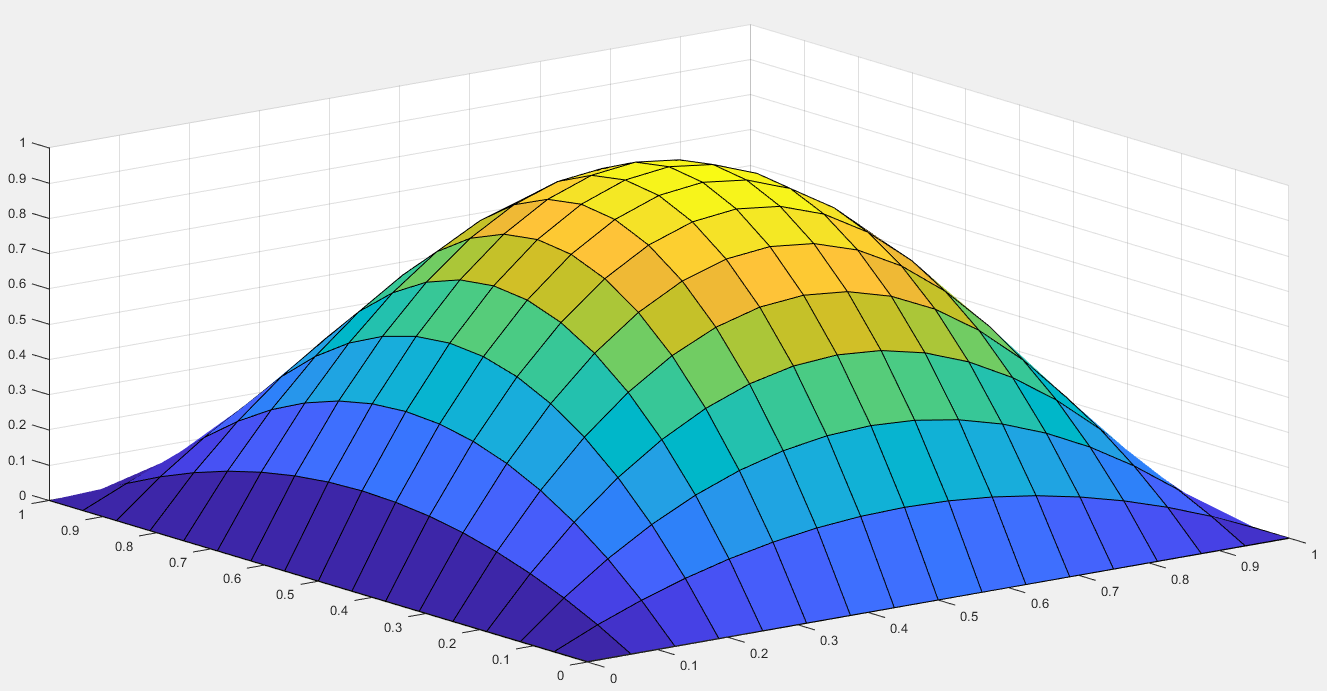
\includegraphics[width=\linewidth]{Aufgaben-Ressourcen/A4L4.png}
		\caption{l=4; h=1/16;}
		\label{A4L4}
	\end{figure}
\begin{figure}
		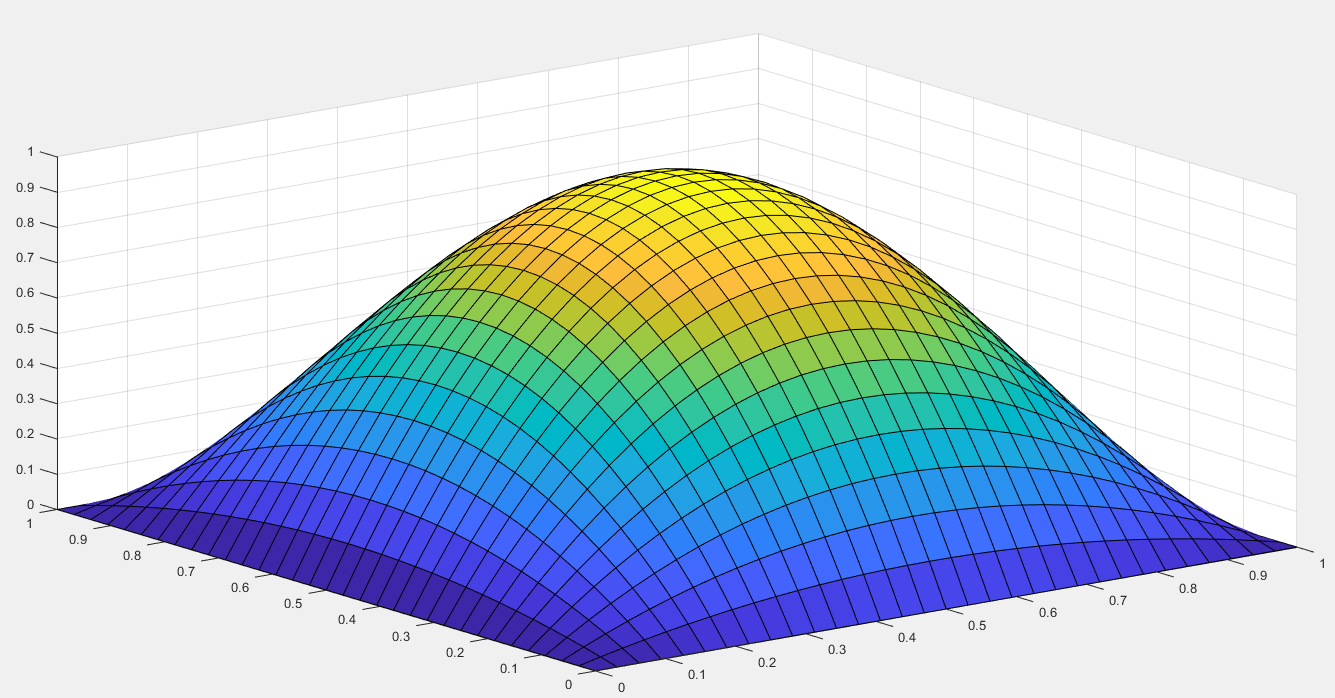
\includegraphics[width=\linewidth]{Aufgaben-Ressourcen/A4L5.png} 
		\caption{l=5; h=1/32;}
		\label{A4L5}
	\end{figure}
	\begin{figure}
		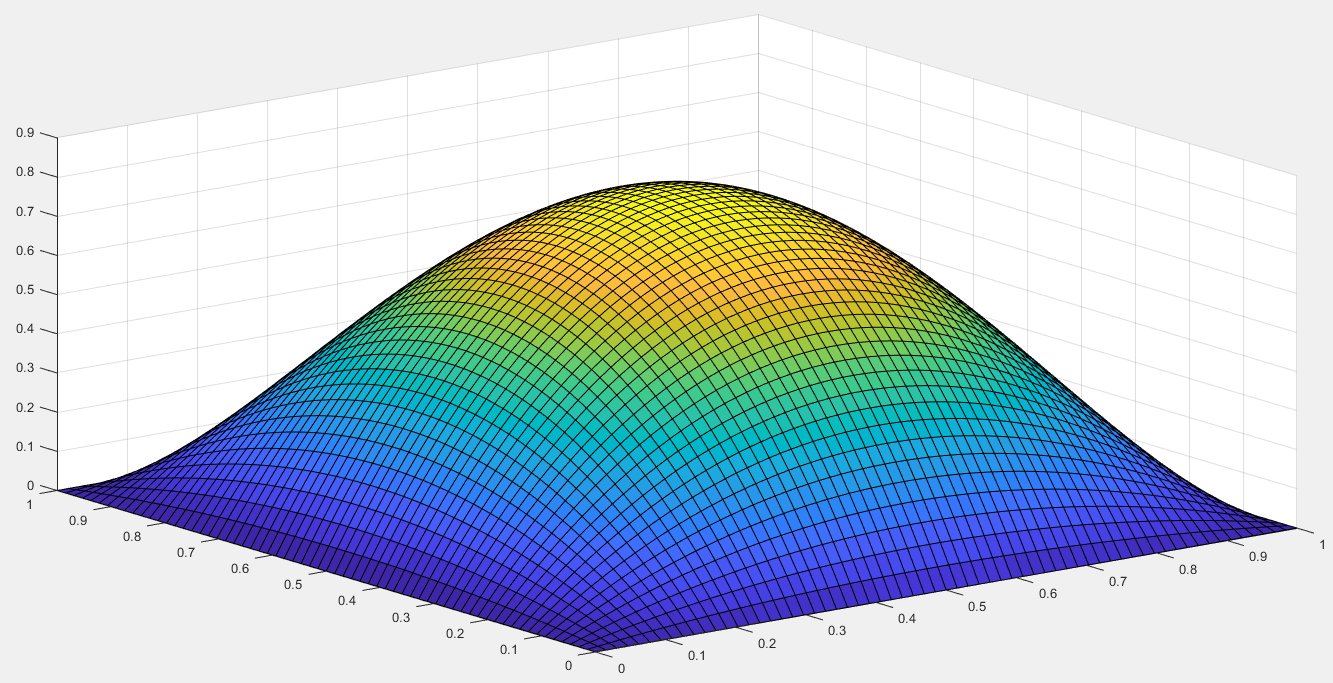
\includegraphics[width=\linewidth]{Aufgaben-Ressourcen/A4L6.png} 
		\caption{l=6; h=1/64;}
		\label{A4L6}
	\end{figure}


	\subsubsection{a)}
Alle Programmdurchläufe für die Messungen hatten eine Fehlerschranke von 0.000001.\newline
\begin{tabular}{|l|l|r|r|}
		\hline
		- & l=4; h=1/16 & l=5; h=1/32 & l=6; h=1/64\\
		\hline
		& 0.050s & 1.429s & 37.296s \\
		& 0.041s & 1.426s & 37.014s  \\
		& 0.040s & 1.392s & 37.061s \\
		& 0.037s & 1.428s & 37.416s  \\
		& 0.051s & 1.424s & 37.295s  \\
		& =0.044s & =1.420s & =37.216s  \\
		\hline

	\end{tabular}
	\newline Diese Lösungswerte in Figure \ref{A4L4}, \ref{A4L5} und \ref{A4L6} ergeben sich mit l=4,5,6;  \newline
	
	\subsubsection{b)}
	Die Schleifenabläufe sind direkt voneinander abhängig und müssen in Reihenfolge ablaufen. Die naive Parallelisierung liefert keine korrekten Ergebnisse. 
	

	\subsubsection{c)}
		Methodik: Die beiden Summen die innerhalb der Schleife berechnet werden müssen wurden parallelisiert und mit einer Reduktion zusammendgefasst.\newline
		\begin{tabular}{|l|l|r|r|r|}
				\hline
				&Laufzeit(seriell) &Laufzeit(parallel) & SpeedUp & Efficiency\\
			\hline
			l=4; h=1/16 & 0.044s & 0.242s & 0.182 & 0.004 \\
			l=5; h=1/32 & 1.420s & 1.154s & 1.231 & 0.026 \\
				l=6; h=1/64 & 37.216s & 26.884s & 1.384 & 0.029 \\
				\hline

		\end{tabular}


    \subsection{Aufgabe 5}
	\begin{figure}
		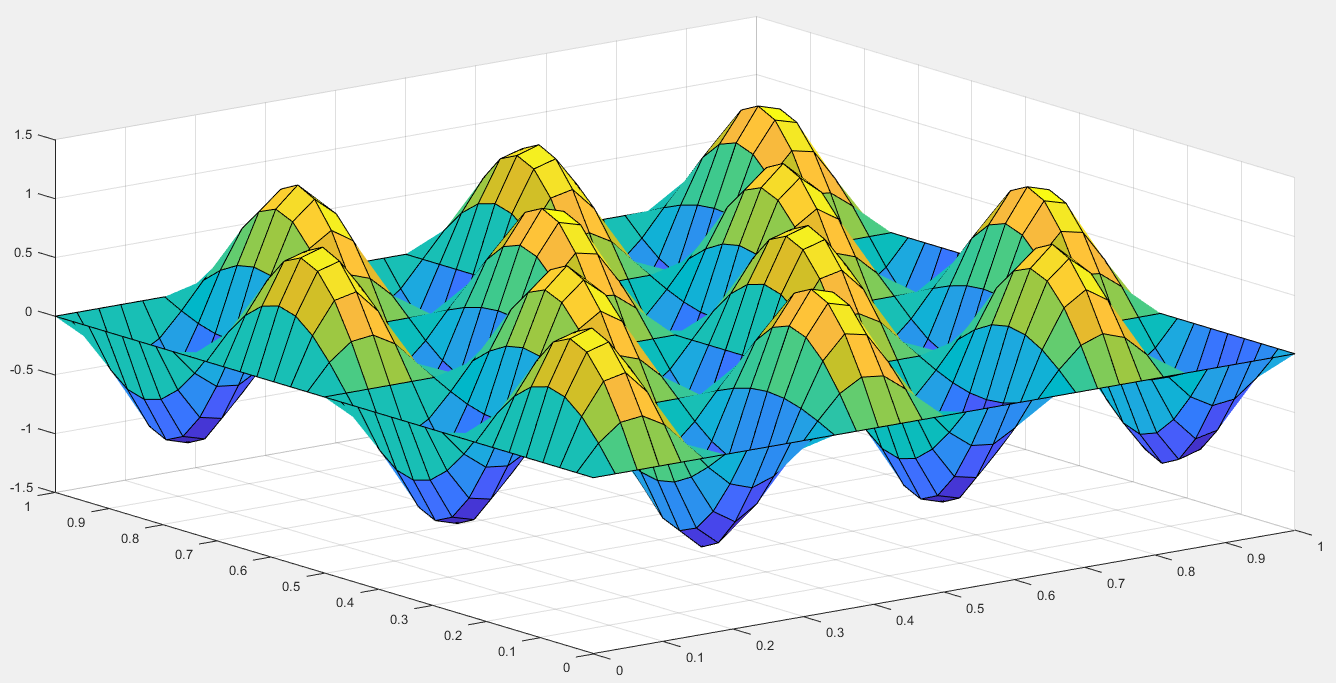
\includegraphics[width=\linewidth]{Aufgaben-Ressourcen/A5L5M3N2.png} 
		\caption{l=5; h=1/32;}
		\label{A5L5}
	\end{figure}
	\begin{figure}
		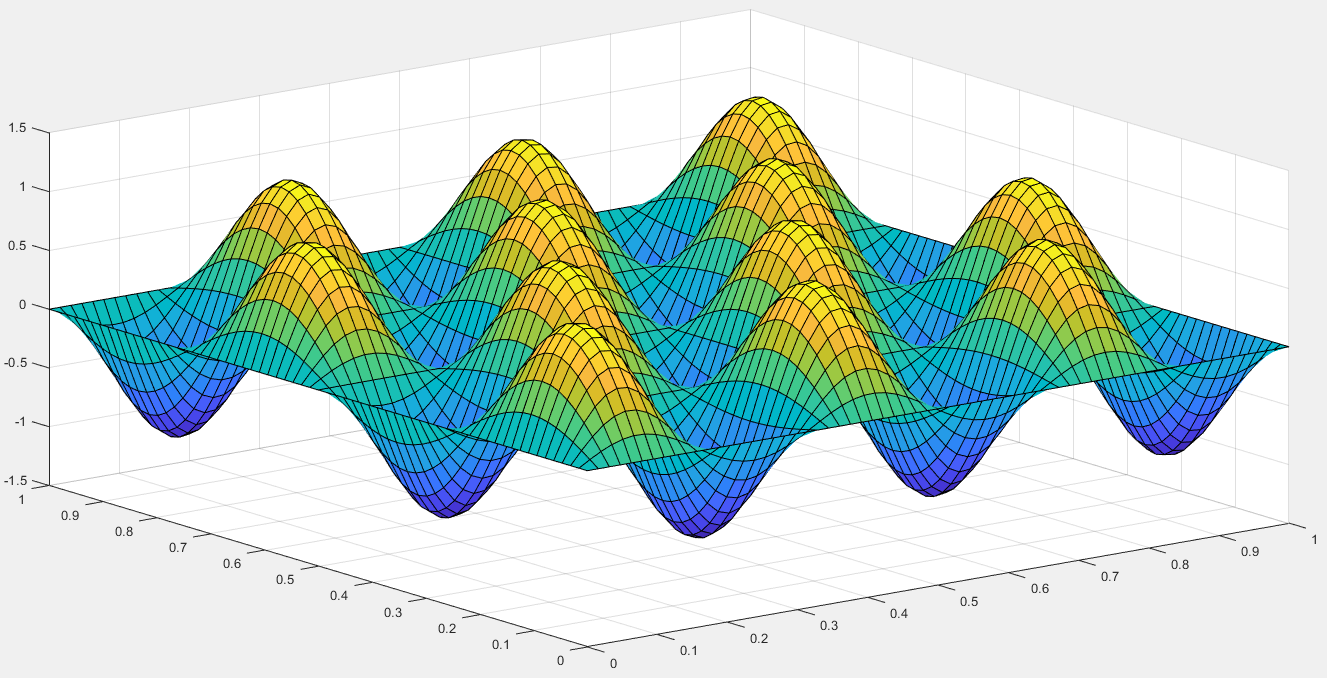
\includegraphics[width=\linewidth]{Aufgaben-Ressourcen/A5L6M3N2.png} 
		\caption{l=6; h=1/64;}
		\label{A5L6}
	\end{figure}
	\begin{figure}
		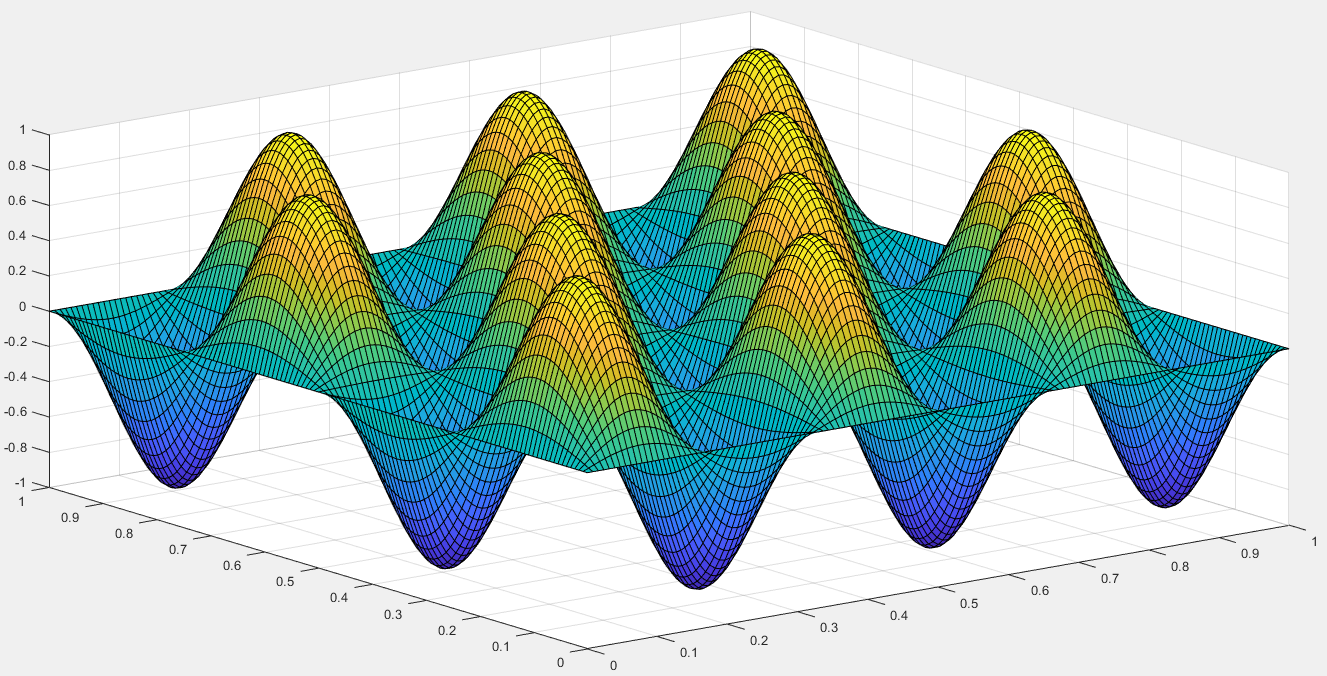
\includegraphics[width=\linewidth]{Aufgaben-Ressourcen/A5L7M3N2.png}
		\caption{l=7; h=1/128;}
		\label{A5L7}
	\end{figure}
	\subsubsection{a)}
	f(x,y) muss definiert sein auf $\Omega$ \newline
	$\Gamma$ ist der Rand von $\Omega$  \newline
	L\"{o}sung u(x,y) muss zweifach differenzierbar sein 
	\subsubsection{b)}
	f(x,y) = ($N^2$ + $M^2$)*4*$\pi^2$*sin(2*M*$\pi$*x)*sin(2*N*$\pi$*y)
	\subsubsection{c)}
	Es handelt sich um eine h-FEM.  \newline
	Die Lösungswerte in Figure \ref{A5L5}, \ref{A5L6} und \ref{A5L7} ergrben sich mit M=3; N=2; l=5,6,7;  \newline


\subsection{Aufgabe 6}
\begin{figure}
	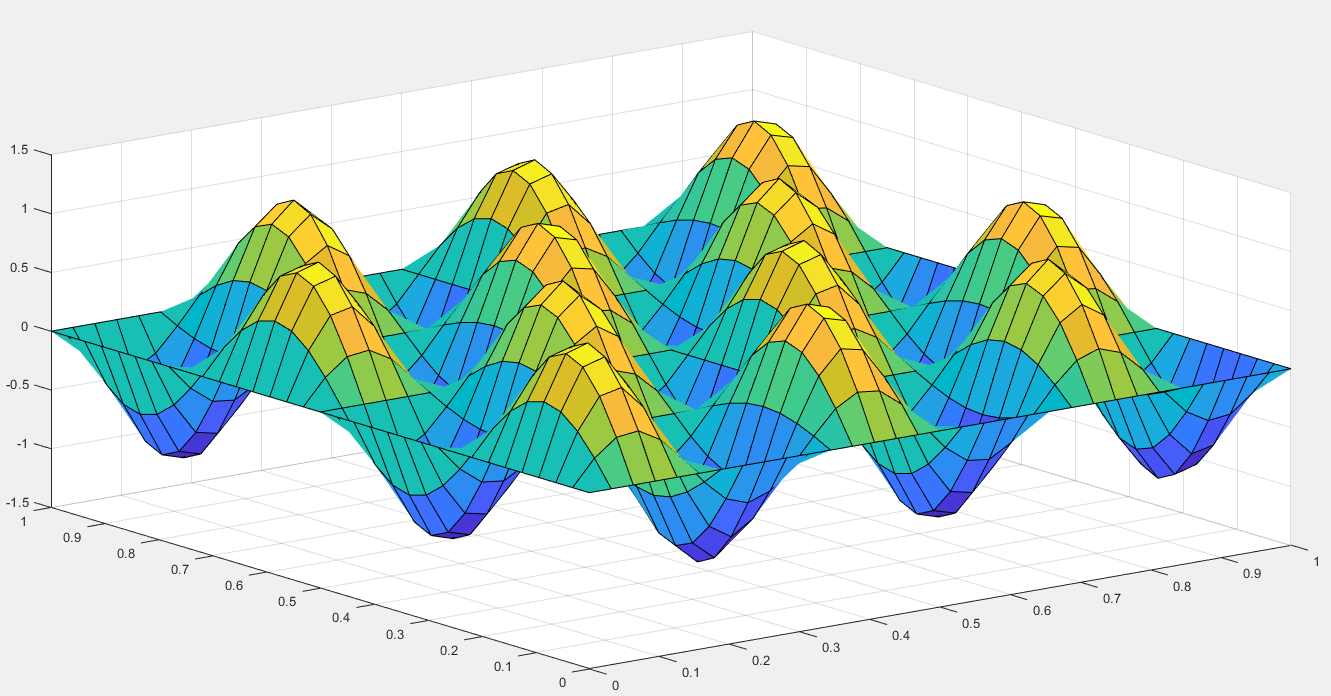
\includegraphics[width=\linewidth]{Aufgaben-Ressourcen/A6L5M3N2.png} 
		\caption{GMRES; l=5; h=1/32;}
		\label{A6L5}
\end{figure}
\begin{figure}
	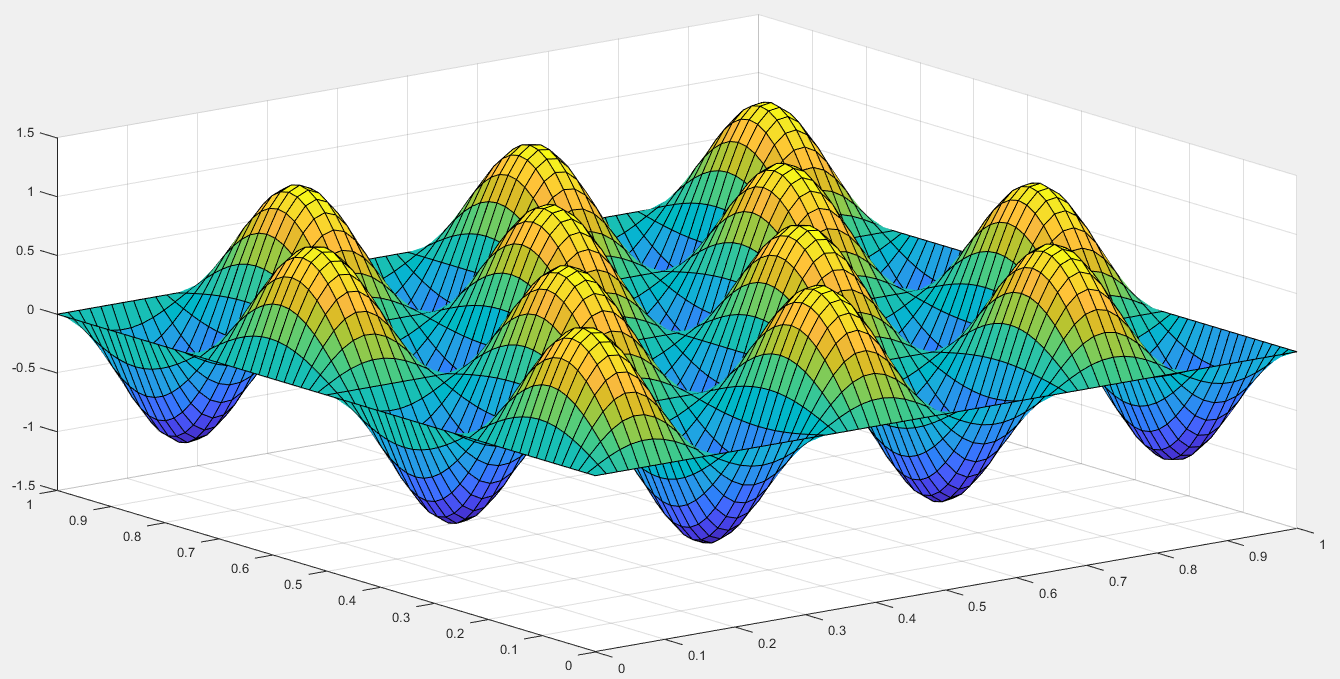
\includegraphics[width=\linewidth]{Aufgaben-Ressourcen/A6L6M3N2.png} 
		\caption{GMRES; l=6; h=1/64;}
		\label{A6L6}
\end{figure}
\begin{figure}
	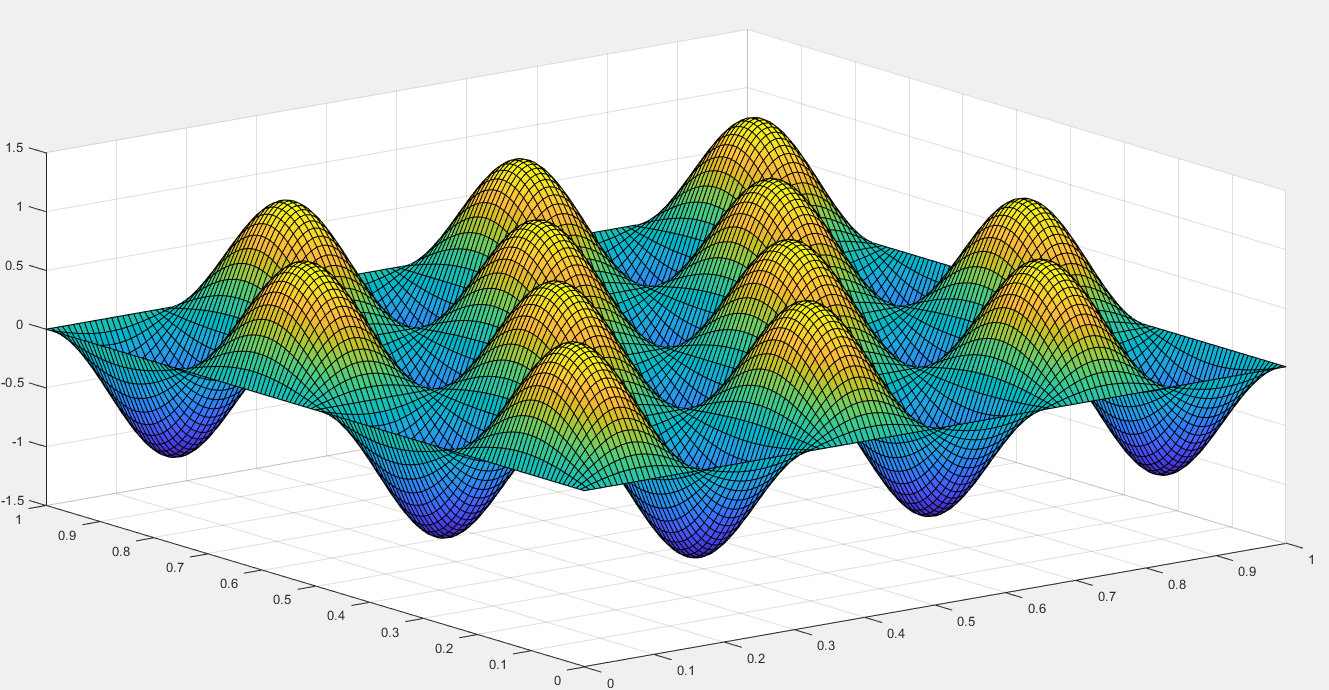
\includegraphics[width=\linewidth]{Aufgaben-Ressourcen/A6L7M3N2.png}
		\caption{GMRES; l=7; h=1/128;}
		\label{A6L7}
\end{figure}
	\subsubsection{a)}
	Liste: CG Verfahren; PCG-Verfahren; Verfahren der minimalen Risiduen(GMRES); GCR-Verfahren; Arnoldi-Verfahren; FOM, ORTHORES;\newline
	Das Gleichungssystem ist dünnbesetzt und alle Krylow-Unterraumverfahren sind gut geeignet f\"{u}r d\"{u}nnvesetzte Gleichungssysteme.
	Diese Lösungswerte in Figure \ref{A6L5}, \ref{A6L6} und \ref{A6L7} ergeben sich mit der Gleichung aus Aufgabe 5 und M=3; N=2; l=5,6,7;  \newline

	\subsubsection{b)}
	Die Verwendung des Residuums als Abrruchbedingung ist eventuell problematisch, da man dadurch in jedem Schleifendurchlauf einen Lösungsvektor $x^k$ berechnen muss. Man kann sich eine feste Anzahl von Iterationen setzen, allerdings hat man dann keine garantierte Genauigkeit. Außerdem kann man das Residuum mit weniger Rechenaufwand in jeder Iteration abschätzen und diesen Schätzwert als Abbruchbedingung nutzen. Auch diese Vorgehensweise hat keine garantierte Genauigkeit, da die Schätzgenauigkeit variiert. Im Zuge des Praktikums haben wir bis jetzt nur eine stabile Version mit abgeschätztem Residuum implementiert(gmres.c). Die Version mit dem Residuum als Abbruchbedingung funktioniert nicht verlässlich(gmresResiduum.c).
	\subsubsection{c)}
Die Efficiency ist bei jedem Vergleich zwischen Aufgabe 6 und Aufgabe 5c gleich dem Speedup, da die Anzahl N der Kerne auf denen das Programm läuft nicht variiert.\newline
\begin{tabular}{|l|l|r|r|}
		\hline
		- & Aufgabe 5(s) & Aufgabe 6(s) & Speedup\\
		\hline
		l=5; h=1/32 &  +1.450 & +0.028 & 56.96 \\
		& +1.420 & +0.021 &    \\
		& +1.371 & +0.026 &    \\
		& +1.475 & +0.026 &    \\
		& +1.408 & +0.026 &   \\
		&=1.424 & =0.025  & \\
		\hline
		l=6; h=1/64 &  +15.427 & +0.140 & 98.488 \\
		& +12.546 & +0.148 &    \\
		& +12.561 & +0.089 &    \\
		& +12.766 & +0.142 &    \\
		& +13.081 & +0.155 &   \\
		&=13.276 & =0.135  & \\
		\hline
		l=7; h=1/128 &  +107.183 & +1.289 & 81.113 \\
		& +105.581 & +1.188 &    \\
		& +104.562 & +1.175 &    \\
		& +105.834 & +1.703 &    \\
		& +104.077 & +1.148 &   \\
		&=105.447 & =1.300  & \\
		\hline
	\end{tabular}
\newline
Einsatz eines Vorkonditionierers: Der Einsatz ist unsinnvoll, da wir bereits eine d\"{u}nn besetzte Matrix gegeben haben. Falls die Matrix anders besetzt wäre, könnte ein Vorkonditionierer von Nutzen sein.
	\subsubsection{d)}
MFEM; deal.II; libMesh; JuliaFEM; FEniCS; Hermes Project;...\newline
Liste weiterer FEM Packages/Libraries: https://en.wikipedia.org/wiki/List\_of\_finite\_element\_software\_packages \newline
Fast alle sind Open Source und kostenlos nutzbar. "Hermes Project" scheint zum Beispiel eine leicht nutzbare C/C++ Bibliothek.

\newpage

\section{Aufgabenblatt 2}

\subsection{Aufgabe 1}

Es gibt sehr viele Eigenschaften die man auslesen kann. Hier sind mögliche Ausgaben: \\

Number of Devices: 2\\
Device Number:                0\\
Device Name:                  Tesla K80\\
Memory Clock Rate (KHz):      2505000\\
Memory Bus Width (bits):      384\\
Global Memory size (bytes):   11996954624\\
Device Number:                1\\
Device Name:                  Tesla K80\\
Memory Clock Rate (KHz):      2505000\\
Memory Bus Width (bits):      384\\
Global Memory size (bytes):   11996954624\\

\subsection{Aufgabe 2}

\paragraph{Arraygröße} Bei kleinen Arrays lohnt sich Cuda nicht wirklich zur Steigerung der Transferrate (Zu viel Overhead?).
Wenn die Arrays sehr groß werden beobachtet man jedoch eine deutliche Steigerung der Effizienz.
Hier wurde mit nvprof gemessen.

\begin{center}
	\begin{tabular}{|l|l|l|l|l|}
		\hline
		N         & Device to Host     & Host to Device     & Device to Device     & Host to Host      \\ \hline \hline
		10			& 2.1120us & 2.0160us &  3.7440us & 3.000us \\ \hline
		100			& 2.3360us & 2.0800us  & 3.8400us & 4.000us\\ \hline
		1000	& 2.6880us & 2.5280us & 3.5200us & 3.000us \\ \hline 
		10000     & 7.4240us & 10.368us & 3.2640us & 22us      \\ \hline
		100000    & 55.679us & 58.240us & 7.7760us & 156us     \\ \hline
		1000000   & 624.25us & 553.79us & 74.015us & 2.171ms   \\ \hline
		10000000  & 5.4335ms & 5.3853ms & 621.02us & 25.503ms  \\ \hline
		100000000 & 53.996ms & 54.383ms & 6.1003ms & 266.338ms \\ \hline
	\end{tabular}
\end{center}

\paragraph{Werte um X erhöhen} 

\begin{center}
		\begin{tabular}{|c|l|l|}
		\hline                                                                             
		\multicolumn{1}{|l|}{blocksize}           & N         & Time     \\ \hline
		\multirow{5}{*}{4}                        & 10000     & 14.752us                                                     \\ \cline{2-3} 
		& 100000    & 121.47us                                                                                \\ \cline{2-3} 
		& 1000000   & 1.4293ms                                                                             \\ \cline{2-3} 
		& 10000000  & 14.122ms                                                                              \\ \cline{2-3} 
		& 100000000 & 141.23ms                                                        \\ \hline
		\multirow{5}{*}{8}                        & 10000     & 8.9920us                               \\ \cline{2-3} 
		& 100000    & 62.207us                                                                                \\ \cline{2-3} 
		& 10000000  & 7.0312ms                                                                                  \\ \cline{2-3} 
		& 100000000 & 70.966ms                                                                                \\ \hline
		\multirow{5}{*}{16}                       & 10000     & 5.8880us                                                                                   \\ \cline{2-3} 
		& 100000    & 32.896us                                                                                  \\ \cline{2-3} 
		& 1000000   & 357.12us                                                                                   \\ \cline{2-3} 
		& 10000000  & 3.5412ms                                                                                   \\ \cline{2-3} 
		& 100000000 & 35.236ms                                                                                   \\ \hline
		\multirow{5}{*}{24}                       & 10000     & 4.8000us                                                                                   \\ \cline{2-3} 
		& 100000    & 23.936us                                                                                   \\ \cline{2-3} 
		& 1000000   & 251.20us                                                                                  \\ \cline{2-3} 
		& 10000000  & 2.5063ms                                                                                  \\ \cline{2-3} 
		& 100000000 & 24.878ms                                                                                 \\ \hline
		\multirow{5}{*}{32}             & 10000     & 4.0960us                                                                                   \\ \cline{2-3} 
		& 100000    & 17.920us                                                                                   \\ \cline{2-3} 
		& 1000000   & 184.29us                                                                                   \\ \cline{2-3} 
		& 10000000  & 1.8227ms                                                                                   \\ \cline{2-3} 
		& 100000000 & 18.020ms                                                                                  \\ \hline
	\end{tabular}
\end{center}

\paragraph{Speedup} 
VectorIncrement um 1 nur auf der CPU mit Openmp:\\
N = 10000000:  Im Schnitt 49.6942 ms (zwischen 194 und 440 ms)\\
N = 100000000: 488.84 ms

\begin{center}
	\begin{tabular}{l|l|l|}
		\cline{2-3}
		& \multicolumn{2}{c|}{Speedup} \\ \hline
		\multicolumn{1}{|l|}{blocksize} & N = 10ˆ7      & N = 10ˆ8     \\ \hline
		\multicolumn{1}{|l|}{4}         & 3.52          & 3.49         \\ \hline
		\multicolumn{1}{|l|}{8}         & 7.07          &              \\ \hline
		\multicolumn{1}{|l|}{16}        & 14.03         &              \\ \hline
		\multicolumn{1}{|l|}{24}        & 19.82         &              \\ \hline
		\multicolumn{1}{|l|}{32}        & 27.19         & 27.74        \\ \hline
	\end{tabular}
\end{center}

\subsection{Aufgabe 3}

\subsubsection{a)}

Running with 32 threads.\\
h = 0.015625, n = 63, l = 6\\
~ 6.725816\\
		\begin{tabular}{|l|l|l|r|r|r|}
	\hline
	&Laufzeit(seriell) &Laufzeit(Openmp)& Laufzeit(CUDA) & S (omp) & S (cuda)\\
	\hline
	l=4; h=1/16 & 0.044s & 0.242s & ? & 0.182 & 0.004 \\
	l=5; h=1/32 & 1.420s & 1.154s & ? &1.231 & 0.026 \\
	l=6; h=1/64 & 37.216s & 6.725816 ms & ? & 1.384 & 0.029 \\
	\hline
	
\end{tabular}

\subsubsection{b)}

\subsubsection{c)}

\subsection{Aufgabe 4}

\subsubsection{a)}

\subsubsection{b)}

\subsubsection{c)}

\subsubsection{d)}

\subsection{Aufgabe 5}



\end{document}
